\section{MARCO TEÓRICO}


\subsection{Sistemas de texto a voz}

\subsubsection{Síntesis concatenativa y paramétrica}
La síntesis del habla consiste en la tarea de generar discurso humano, a partir de alguna entrada arbitraría. Son de particular interés para desarrollar interfaces de comunicación entre humanos y computadoras, los sistemas de texto a voz, o TTS (text to speech system). 
Históricamente se emplearon dos metodologías para llevar a cabo esta tarea: La síntesis concatenativa, donde distintos fonemas y palabras pre-grabadas son utilizadas para completar una frase solicitada, y la síntesis paramétrica, donde un modelo acústico es condicionado para modificar nuevamente voces pre-grabadas de acuerdo a variables arbitrarias solicitadas por un usuario. En ambos casos es necesario almacenar fonemas o palabras pre-grabadas, y la calidad de la voz resultante no es ideal, exhibiendo una característica “roboticidad''. Es aquí donde entran en juego técnicas de síntesis basadas en el aprendizaje profundo neuronal, o Deep Learning

%Estas diferencias son ilustradas en la Figura \eqref{fig:redes_capas}.
%
%
%\begin{figure}[H]
%    \centering
%    \includegraphics[scale=.4]{imagenes/Red-neuronal-artificial-de-cuatro-capas.png}
%    \caption{ Red neuronal artificial de cuatro capas. \\
%    (Imágen obtenida de \textit{Alvarado, Matías & Meneses-Bautista, Francisco. (2017). Pronóstico del tipo de cambio USD/MXN con redes neuronales de retropropagación. Research in Computing Science. 113. 97 - 110. %10.13053/rcs-139-1-8}). }
%    \label{fig:redes_capas}
%\end{figure}
%
\subsubsection{Aprendizaje profundo neuronal aplicado a TTS}
A partir de 2016 el campo de los TTS fue revolucionado por distintas arquitecturas basadas en Deep Learning, que mejorarían considerablemente la calidad de las voces sintetizadas. Previo a adéntranos en una breve explicación detrás del funcionamiento de las distintas arquitecturas, podemos observar como un sistema TTS puede ser formulado matemáticamente a partir de la siguiente ecuación:

\begin{equation}
X = argmax P(X | Y, \theta )
\end{equation}

Dado X, el habla sintetizada objetivo, Y la secuencia de caracteres que compone el texto de entrada y \begin{math} \theta \end{math} los parámetros del modelo. Normalmente las distintas metodologías implementadas en esta tarea dividen el labor en dos partes:

\begin{itemize}
    \item Un primer modelo que se encarga de generar las características acústicas de la voz a sintetizar. Es común que se obtenga un espectrograma como la salida de esta primer parte del sistema.
    \item Un vocoder, o codificador de voz, también basado en redes neuronales es utilizado para generar en una segunda instancia la voz sintetizada. Es normal que esta parte de generación de señal audible este acompañada por distintos algoritmos de mejora del habla (speech enhancement).
\end{itemize}

Posterior a esto, es común incluir una etapa de post-procesado, implementando distintos filtros y el re-sampleo de la señal, que pueden ayudar a disminuir artefactos y otros tipos de ruidos e imperfecciones generados durante la inferencia de voz.

\subsection{Evaluación de voces sintetizadas}

Mean Opinion Score (MOS) \cite{itu}, o promedio de la puntuación subjetiva, en castellano, es una métrica que proviene del campo de las telecomunicaciones utilizada para determinar la “calidad de la experiencia'' de un usuario o conjunto de usuarios, sobre un estimulo o sistema en particular. Normalmente el MOS opera sobre una escala ordinal (símil escala Lickert), típicamente usando un rango discreto entre 1-5, donde las puntuaciones representan una valoración \textbf{Mala} a \textbf{Excelente} (Tabla \eqref{tab:MOS} ), aunque también es posible utilizar otras escalas. 

\begin{table}[h]
\centering
\caption{Posible escala para un MOS}
\label{tab:MOS}
\begin{tabular}{cclll}
\textbf{Puntuación} & \textbf{Calidad} &  &  &  \\ \cline{1-2}
5               & Excelente      &  &  &  \\
4               & Buena           &  &  &  \\
3               & Aceptable           &  &  &  \\
2               & Mediocre           &  &  &  \\
1               & Mala            &  &  & 
\end{tabular}
\end{table}

Uno de los posibles problemas de este tipo de evaluación, es que los sujetos de prueba suelen percibir que los “saltos'' entre cada categoría no son equidistantes (por ejemplo, puede haber una separación más grande entre las valoraciones \textbf{Buena} y \textbf{Excelente}, que entre \textbf{Aceptable} y \textbf{Buena}. Otro sesgo recurrente es el denominado “ecualización de rango'', el cual lleva a sujetos a tratar de utilizar todas las puntuaciones posibles a lo largo de una prueba. En otras palabras, se tiende a querer utilizar todas las puntuaciones posibles al menos una vez. Esto hace que sea imposible comparar la opinión entre dos sujetos de prueba distintos, a menos que el rango de calidad esperada de los ejemplos sea equivalente entre ambas pruebas.

MOS es el test subjetivo más frecuentemente utilizado para determinar la calidad de voces sintetizadas. La prueba presenta una serie de ejemplos que deben ser evaluados por distintos oyentes, de acuerdo a algún parámetro especifico. En general, las voces sintetizadas son juzgadas de acuerdo a su “naturalidad''. La naturalidad de una voz es un termino difícil de definir, muchas metodologías de evaluación subjetiva incluso prefieren no aclarar el significado de dicha variable, proponiendo que sugerirle una definición a los sujetos de prueba puede sesgar la evaluación pretendida. Sin embargo, dentro del alcance de esta investigación, podemos decir que la naturalidad de una voz sintetizada representa un valor que nos informa acerca de que tanto se asemeja esa voz, a la de un humano. El test MOS emplea una escala discreta de 5 puntos (1 a 5), en la cual el discurso humano real se encuentra entre los valores de 4,5 a 4,8. 

Existen distintos modelos de calidad que apuntan a predecir el resultado de un MOS (típicamente desarrollados utilizando el resultado de tests MOS realizados previamente). Algunos ejemplos de estos sistemas, orientados a la calidad de la voz, son desarrollados en la sección 3 de este documento.

\subsection{Técnicas posibles de alteración del hablante}

El proceso conocido como Data Augmentation (DA, o aumento artificial de datos), tiene el objetivo de aumentar la cantidad de información o muestras recolectadas en una base de datos, manteniendo ciertos rasgos elementales de los ejemplos originales, y sin modificar la distribución de la totalidad de las muestras. Para esta investigación, es necesario poder modificar y variar incluso sutilmente las muestras recolectadas con el fin de obtener un espacio de datos más variado. 

\subsubsection{Vocal Tract Lenght Perturbation}
Se propone implementar técnicas de alteración del largo del tracto vocal \cite{vtlp} (Vocal Tract Length Perturbation, VTLP). Dicha técnica fue desarrollada para mejorar sistemas de reconocimiento del habla, e involucra la deformación en espacio y tiempo del espectro de cada audio. El resultado es semejante a un desplazamiento frecuencial, pero el resultado es el de una voz más natural. En la Figura \eqref{fig:vtlp} puede observarse una comparación entre un desplazamiento frecuencial y una transformación VTLP.


\begin{figure}[H]
    \centering
    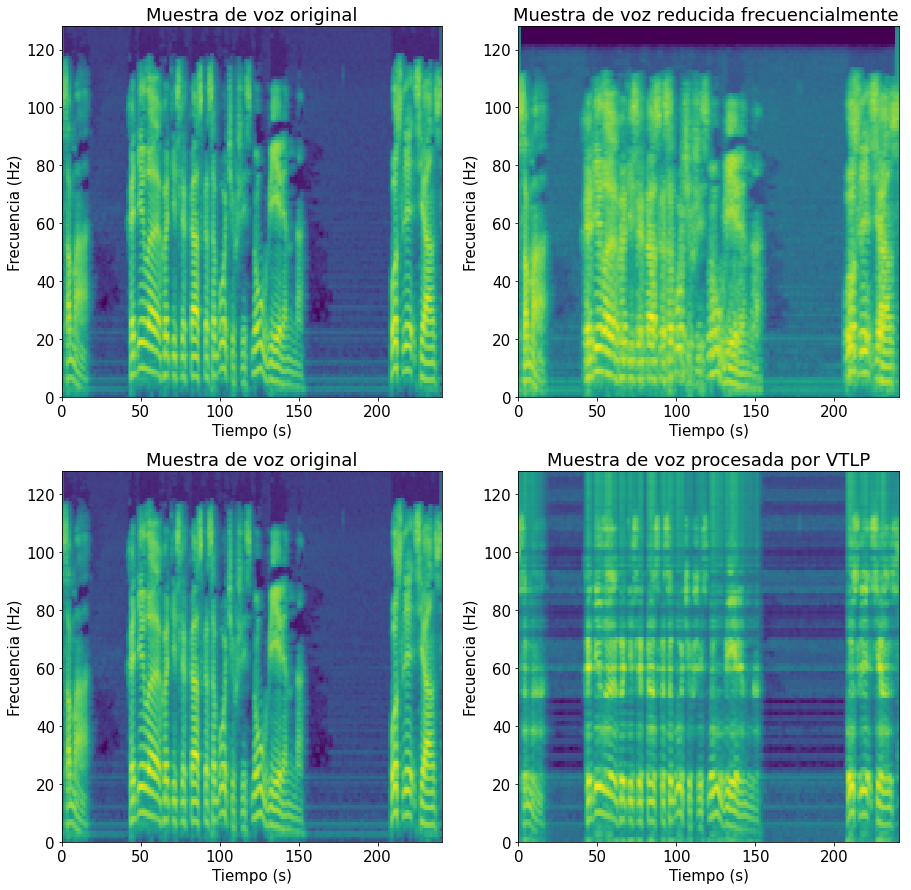
\includegraphics[scale=0.5]{imagenes/vtlp.png}
    \caption{Espectro de una voz modificada frecuencialmente, y mediante una transformación VTLP.}
    \label{fig:vtlp}
\end{figure}

\subsubsection{Algoritmo de Griffin-Lim}
El algoritmo de Griffin-Lim (ALG)\cite{griffin} es un método de reconstrucción de fase para señales de las que únicamente se tiene su componente de magnitud. El método de estimación de fase consiste de los siguientes pasos:

\begin{itemize}
    \item 1. Inicializar la fase aleatoriamente como ruido uniforme.
    \item 2. Realizar la transformada inversa de Fourier (inverse short-time Fourier transform, ISTFT).
    \item 3. Realizar la transformada de fourier (STFT) sobre la señal temporal obtenida. Esto deriva mínima información de fase de la señal temporal.
    \item 4. Reemplazar la magnitud obtenida por la STFT realizada por la magnitud de la señal original. Esto mantiene intacta la información de magnitud de la señal en el espectro, y agrega la minima información de fase de la señal que se deriva de la redundancia de la STFT.
    \item 5. Iterar los pasos 2-5 hasta obtener un resultado satisfactorio.
\end{itemize}
Iteración a iteración la información de fase resultara más pertinente a la componente de magnitud, dato original de la señal en el espectro. Muchos modelos de vocoder ignoran o tienen problemas para modelar la fase de una voz sintetizada. Este algoritmo puede ayudar a recrear en parte los artefactos característicos de algunos sistemas TTS.

\subsection{Vectorización de hablantes (speaker embeddings)}

La extracción de un descriptor numérico de cada audio a evaluar es un proceso necesario para el posterior entrenamiento de la red neuronal que se encargará de calificar cada modelo TTS. Los vectores de hablantes, (Speaker Embeddings) permiten extraer información critica de cada locutor a partir de una representación sonora del mismo, obteniendo un único descriptor capaz de codificar identidad de hablante, genero, velocidad del habla y contenido semántico del texto \cite{SpeakerEmbedding}. El proceso de extracción y la información codificada varía de implementación a implementación.

Los X-Vectors \cite{xvectors}, consisten en una representación vectorizada de cada hablante que aprovecha el uso de técnicas de DA. La representación resultante ha sido útil para mejorar la eficiencia de sistemas de reconocimiento de locutores. Una implementación de la red neuronal que extrae este tipo de descriptor se encuentra disponible en el Kaldi toolkit \cite{kaldi}.

Por otro lado HuBERT \cite{hubert} presenta una metodología auto-supervisada para extraer speaker embeddings. Existen tres problemas principales a la hora de generar este tipo de representaciones a partir de audios de una manera auto-supervisada, es decir, utilizando una base de datos no etiquetada: (1) existen más de una unidad sonora dentro de cada audio a procesar, (2) no existe un vocabulario o léxico de sonidos posibles en la etapa de pre-entrenamiento, y (3) la unidad sonora no tiene una segmentación explicita. Hubert presenta una implementación novedosa para la extracción auto-supervisada de speaker embeddings. Concretamente, el modelo aprende a agrupar (clustering) distintas unidades sonoras, enmascarando parte de la información, similar a la metodología planteada por \textbf{BERT}. La función de perdida se aplica únicamente sobre las regiones enmascaradas, forzando al modelo a aprender representaciones de alto nivel de la parte desenmascarada de la unidad sonora, para poder inferir correctamente respecto de como clasificar las regiones enmascaradas. Hubert extrae tanto información acústica, como lingüística como parte de su proceso de vectorización.

\newpage